% =====================================================================
%  Master Thesis Proposal / Opening Report
%  Zhejiang University, School of Economics
%  Student: Mario Diez Martinez, 22501254
%  Supervisor: Du Limin
%  Formatting authority:
%  ../../08_admin/proposal_defense/zju_thesis_formatting_guidelines.md
%  Overleaf copy: compile with XeLaTeX. Generated by make_overleaf_copy.py.
% =====================================================================
% OVERLEAF-FRIENDLY COPY. Edit main.tex, then regenerate this file.
\documentclass[12pt,a4paper]{article}

\usepackage[margin=2.6cm,top=3cm,bottom=2.5cm]{geometry}
\usepackage{fontspec}
\usepackage[UTF8,fontset=fandol]{ctex}
\setmainfont{TeX Gyre Termes}
\setCJKmainfont[AutoFakeBold=2.0]{FandolFang-Regular}
\usepackage{setspace}
\usepackage{amsmath,amssymb}
\usepackage{chngcntr}
\usepackage{booktabs}
\usepackage{tabularx}
\usepackage{array}
\usepackage{indentfirst}
\usepackage{etoolbox}
\usepackage{float}
\usepackage{caption}
\usepackage{graphicx}
\graphicspath{{figures/}}
\usepackage{pdflscape}
\usepackage{tikz}
\usetikzlibrary{arrows.meta,positioning}
\usepackage{titlesec}
\usepackage[authoryear,round]{natbib}
\usepackage{xurl}
\usepackage[hidelinks,breaklinks=true]{hyperref}
\urlstyle{same}
\emergencystretch=3em

% Keep author-year citations in the text, while printing numbered entries in
% the reference section to match the proposal format.
\makeatletter
\AtBeginDocument{%
  \let\@biblabel\NAT@biblabelnum
  \let\@bibsetup\NAT@bibsetnum
}
\makeatother

\onehalfspacing
\setlength{\parindent}{1.5em}
\setlength{\parskip}{0pt}
\setcounter{secnumdepth}{3}
\setcounter{tocdepth}{3}

% ZJU formatting guideline: headings use FangSong for Chinese, Times New Roman
% for numbers/English, bold, with 1.5 spacing and prescribed before/after space.
\titleformat{\section}
  {\fangsong\bfseries\fontsize{15pt}{22.5pt}\selectfont}
  {\thesection}{0.75em}{}
\titlespacing*{\section}{0pt}{2\baselineskip}{0.5\baselineskip}
\titleformat{\subsection}
  {\fangsong\bfseries\fontsize{14pt}{21pt}\selectfont}
  {\thesubsection}{0.75em}{}
\titlespacing*{\subsection}{0pt}{1\baselineskip}{0.5\baselineskip}
\titleformat{\subsubsection}
  {\fangsong\bfseries\fontsize{12pt}{18pt}\selectfont}
  {\thesubsubsection}{0.75em}{}
\titlespacing*{\subsubsection}{0pt}{0.5\baselineskip}{0pt}

% ZJU formatting guideline: figures, tables, and equations are numbered by
% section/chapter as Figure 1-1, Table 1-1, and (1-1).
\counterwithin{figure}{section}
\counterwithin{table}{section}
\numberwithin{equation}{section}
\renewcommand{\thefigure}{\thesection-\arabic{figure}}
\renewcommand{\thetable}{\thesection-\arabic{table}}
\renewcommand{\theequation}{\thesection-\arabic{equation}}

% ZJU formatting guideline: captions are centered, single-spaced, and close to
% the relevant figure/table. Tables should be source-level caption-above;
% figures should be source-level caption-below.
\captionsetup{
  font={small,stretch=1.0},
  labelfont=bf,
  justification=centering,
  skip=0.5\baselineskip
}
\captionsetup[table]{position=top}
\captionsetup[figure]{position=bottom}

% ZJU formatting guideline: use full-width three-line tables without vertical
% rules. booktabs implements the required top, middle, and bottom rules.
\setlength{\heavyrulewidth}{1.2pt}
\setlength{\lightrulewidth}{0.75pt}
\setlength{\cmidrulewidth}{0.75pt}
\AtBeginEnvironment{tabular}{\small}
\AtBeginEnvironment{tabularx}{\small}

\setlength{\abovedisplayskip}{0.5\baselineskip}
\setlength{\belowdisplayskip}{0.5\baselineskip}
\setlength{\abovedisplayshortskip}{0.5\baselineskip}
\setlength{\belowdisplayshortskip}{0.5\baselineskip}

\renewcommand{\bibsection}{%
  \par\vspace{2\baselineskip}%
  \begin{center}
    {\fangsong\bfseries\fontsize{15pt}{22.5pt}\selectfont References}
  \end{center}
  \vspace{0.5\baselineskip}%
}

\newcommand{\makezjucover}{%
\begin{titlepage}
\thispagestyle{empty}
\begin{tikzpicture}[remember picture,overlay]
  \node[anchor=center, inner sep=0pt] at (current page.center)
    {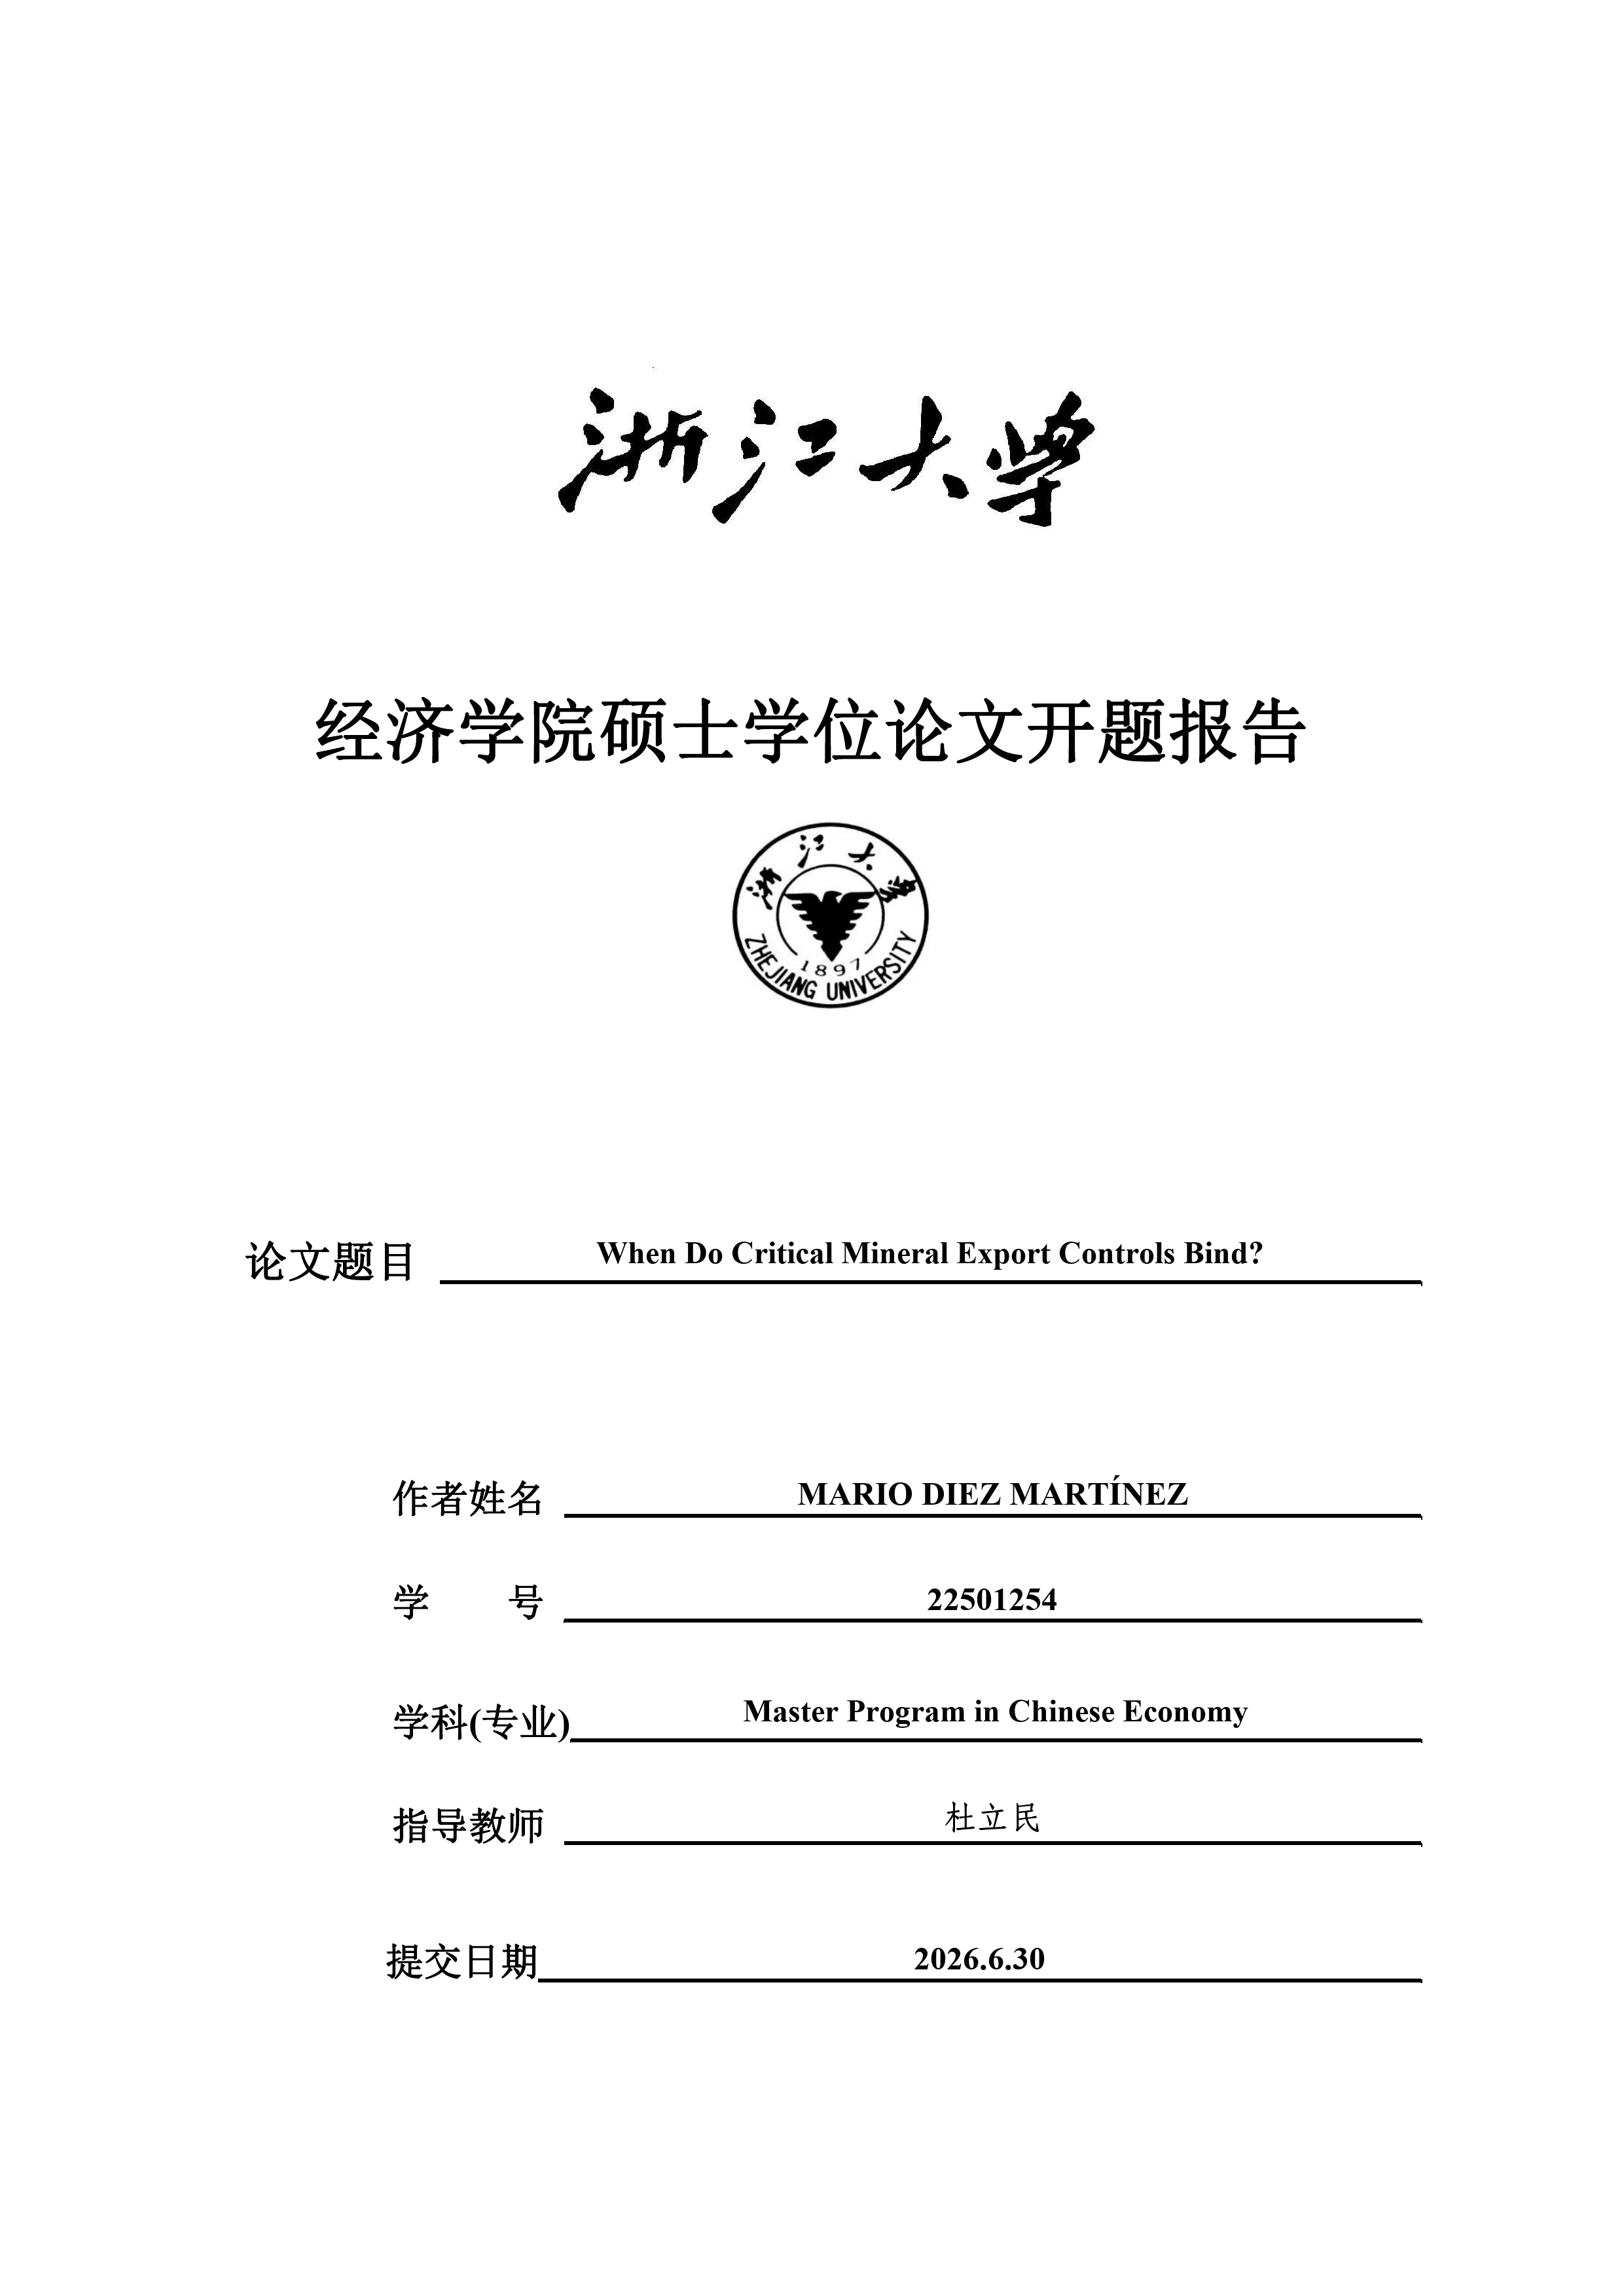
\includegraphics[width=\paperwidth,height=\paperheight]{cover_assets/zju_cover_mario.png}};
\end{tikzpicture}
\null
\end{titlepage}
}

\begin{document}

\makezjucover

{\footnotesize
\tableofcontents
}
\newpage

\section{Research Background and Significance}

\subsection{Research Background}

\subsubsection{Critical Minerals, Supply Chains, and Economic Statecraft}

Critical minerals are inputs for semiconductors, batteries, defense systems, renewable energy equipment, and other strategic industries. Their supply chains are often concentrated in a small number of mining, refining, or processing locations. China occupies a central position in many of these markets, especially in refining, processing, and intermediate material supply. Economic statecraft means the use of economic policy tools to pursue strategic or political goals. In this setting, the tool is export licensing, and the channel is access to Chinese supply. A licensing rule can change importers' sourcing choices, shipment timing, price exposure, and risk in supply chains.

The economic statecraft literature shows that states can use central positions in global networks to create chokepoints and shift costs onto foreign actors \citep{farrell2019weaponized,egger2024sanctions}. Critical minerals are a physical supply chain setting for the same broad problem. Unlike financial or digital networks, critical mineral networks move through mines, refineries, processors, traders, and downstream users. The relevant issue is when control over a concentrated production or processing node produces an observable trade or price response.

Critical mineral market power is difficult to measure directly. A country can dominate mining, processing, refining, or one narrow grade without controlling every trade flow recorded under a broad customs code. An importer can also reduce Chinese sourcing without reducing total imports if non-China supply is available. Dependence on Chinese supply is therefore a market condition, not the outcome. The outcome is the observed adjustment after a licensing rule takes effect.

The policy setting is also different from technology controls on demand. A semiconductor export control may restrict foreign access to a technology, equipment, or supply chain tied to a specific firm. A mineral export license restricts access to upstream or midstream material that enters many downstream uses. The same license can affect defense producers, battery firms, chemical users, traders, and inventory holders in different ways. This makes the product and source margins central. The empirical problem is not only whether a mineral was covered by a control. The trade data require the analysis to ask which Harmonized System (HS) code records the controlled item, which source is affected, which importers adjust, and when the change appears.

China's market share alone does not determine the trade effect. Market share creates potential pressure, but the realized effect depends on product scope, HS code measurement, importer exposure, outside suppliers, and demand conditions. International organizations now track export restrictions on critical raw materials as a growing policy issue, but those inventories mainly describe policy use and market exposure \citep{oecd2026_crm_export_restrictions,iea_2025_global_critical_minerals_outlook}. They do not show when a specific licensing rule binds in trade data.

\subsubsection{China's Critical Mineral Export Licensing Controls}

China's recent critical mineral measures use export licensing. The Export Control Law gives China a legal basis for controlled items, temporary controls, licensing review, end use and end user documentation, and customs checks \citep{prc_2020_export_control_law}. The State Council white paper presents export controls as part of China's national security, nonproliferation, and international obligation framework \citep{scio_2021_chinas_export_controls}. The 2024 dual use regulation further specifies licensing procedures, review conditions, documentation, and customs release rules for controlled dual use items \citep{prc2024_dual_use_regulations}.

The recent chronology has several mineral waves. China announced controls on gallium and germanium items in July 2023, effective August 1, 2023; graphite items in October 2023, effective December 1, 2023; and antimony and related items in August 2024, effective September 15, 2024 \citep{mofcom_2023_gallium_germanium_controls,mofcom_2023_graphite_controls,mofcom_2024_antimony_controls}. China then announced controls on exports of relevant dual use items to the United States in December 2024, added controls on tungsten, tellurium, bismuth, molybdenum, and indium items in February 2025, and adjusted part of the U.S. measure in November 2025 \citep{mofcom_2024_us_controls_critical_minerals,mofcom_2025_w_te_bi_mo_in_controls,mofcom_2025_suspend_us_controls_art2}. These official documents provide dates, product language, and legal scope. They do not show whether trade changed.

The legal form matters. Export licensing is an authorization procedure, and the non tariff measure literature separates licensing from export prohibitions and quotas \citep{unctad2019ntm_classification,gamberale_tarasenko2023_export_licensing}. The Chinese notices require exporters to apply for licenses for covered items. Official statements on gallium/germanium, graphite, and antimony also indicate that applications could be approved or reviewed under the licensing regime \citep{mofcom_2023_gallium_germanium_approvals,mofcom_2024_graphite_approvals,mofcom_2024_antimony_license_review}. These statements do not report approval rates, processing times, or shipment outcomes. They only show that the instrument was licensing rather than an automatic embargo.

Licensing status and trade effects are different objects. A binding licensing control may reduce imports from China, delay arrivals, increase reliance on non-China suppliers, widen domestic and international price gaps, or affect only the subset of products that closely matches the legal scope. A weakly observed control may show no aggregate HS-level decline even if some controlled items are affected. The empirical object is the trade and price margin after the rule, not an assumed collapse.

A licensing control can affect trade without stopping all shipments. If authorization is slow, uncertain, or document intensive, importers may change suppliers, shipment timing, or inventory before a denial occurs. Administrative delay and shipping time are trade costs, and policy uncertainty can change firm behavior before outcomes are known \citep{djankov_freund_pham2010_trading_on_time,hummels_schaur2013_time_trade_barrier,handley_limao2017_policy_uncertainty}. Customs records may therefore show switching, delay, or price pressure rather than zero exports. For this reason, binding is defined through observable market response rather than through the legal label alone.

\subsection{Research Problem}

Formally similar licensing rules can produce different trade responses across minerals. A licensing control may look similar across episodes, but the market response depends on product scope, HS code aggregation, dependence on China before the policy, outside supplier options, downstream demand, and the credibility of sustained enforcement. Without separating these margins, trade changes after the policy can be misread as either uniform export control success or simple policy irrelevance.

This study addresses this problem by treating the policy as a potential China specific licensing wedge. The wedge is not directly observed. It must be inferred from trade timing, source composition, total import adjustment, domestic and international price differences, and importer heterogeneity.

The research problem has three parts. The first is the legal rule: which items China formally places under export licensing. The second is the trade data unit: whether the available HS code closely records those controlled items or bundles them with other goods. The third is the market response: whether importers reduce China sourcing, switch to non-China suppliers, reduce total imports, or face higher prices. The analysis must keep these parts separate. A legal control does not automatically imply a trade effect, and an HS-level null does not prove that the controlled item was unaffected.

The main research question is: why do formally similar Chinese export licensing controls generate different trade and price disruptions across critical minerals? This study asks whether treated products show a China source decline after the expected import effect month, whether importers switch to non-China suppliers or reduce total imports, and whether price wedges or importer heterogeneity support the interpretation of a trade binding licensing wedge.

\subsection{Research Significance}

The study matters for three reasons. First, it clarifies the trade effect of supply side economic statecraft. Export controls are now central to technology competition, as shown by the semiconductor control literature, but the critical mineral case differs because the policy acts through physical supply chains and licensing requirements that vary by product \citep{bown2020semiconductor,bown2024semiconductors}. The relevant evidence is therefore observable trade adjustment, not the announcement alone.

Second, the study improves measurement. Critical mineral security policy often treats Chinese export controls as a direct proxy for foreign scarcity. That can be misleading. If licensing controls mainly shift sourcing away from China, importing economies face a different problem than if total imports contract. If price wedges widen without large trade declines, quantity data alone understate scarcity. If broad HS codes mix controlled and uncontrolled items, aggregate trade data may hide disruption in the controlled item.

Third, the study is policy relevant for China. Export licensing can create pressure only if it changes the market margin that the policy is meant to affect. A control that leads foreign importers to switch suppliers has a different meaning from a control that reduces total imports, widens price gaps, or shows no detected HS-level response. The analysis does not test coercive success or welfare. It provides product-level evidence on when licensing controls bind, along which margins, and for which types of products and importers.

The policy relevance comes from the difference between exposure and disruption. Exposure shows where China may have potential pressure. Disruption shows where a licensing rule actually changed observed trade. These are not the same. A high China share may not produce a visible import loss if licenses are routine, inventories are large, or the measured HS code is too broad. A lower China share may still matter if the product is hard to replace or if importers have few qualified suppliers. The answer is narrow but useful: which products show observable China source adjustment, and what kind of adjustment is it?

\section{Literature Review}

Four literatures define the gap: economic statecraft, export licensing, mineral adjustment, and empirical trade methods. Together, they show why China's critical mineral controls are a plausible case of supply side economic statecraft. The missing step is product source evidence on when a licensing rule is trade binding.

\subsection{Economic Statecraft and Critical Mineral Controls}

Economic statecraft scholarship starts from asymmetric interdependence. Network power theory argues that states or firms in central positions can turn access to a network into bargaining power, surveillance capacity, or chokepoints \citep{farrell2019weaponized}. Sanctions research reaches a related conclusion from a different setting: coercive economic measures work through exposure, substitutability, adjustment costs, and policy credibility \citep{egger2024sanctions}. These arguments are useful because critical mineral supply chains are concentrated. They are also incomplete for this project because they mainly establish the possibility of leverage, not whether a given product shows a trade response.

The technology control literature gives a closer policy setting. Work on semiconductor controls shows how national security policy can target firms, technologies, and supply chain nodes, and how legal restrictions can reshape commercial choices even outside broad economy wide sanctions \citep{bown2020semiconductor,bown2024semiconductors}. Critical minerals share the strategic input logic, but they differ in where the policy acts. Semiconductor controls often restrict access to advanced technology or equipment. Mineral export controls restrict upstream or midstream material inputs. This difference matters because mineral trade can adjust through source switching, inventory use, price changes, or measurement problems inside broad customs codes.

Critical mineral reports establish the exposure problem but not the realized effect. The IEA emphasizes concentration and diversification as central issues in critical mineral markets \citep{iea_2025_global_critical_minerals_outlook}. The OECD inventory documents the growing use of export restrictions on critical raw materials and classifies licensing as one policy instrument \citep{oecd2026_crm_export_restrictions}. These sources show why the issue matters. They identify exposure and policy use, not realized product source adjustment.

China's export restrictions also belong to a longer legal and political history. Earlier disputes over raw materials and rare earths show that Chinese export restraints have long raised questions about WTO law, industrial policy, and unilateral economic measures \citep{bogdanova_wang2023_china_export_restrictions_wto}. The recent critical mineral controls fit this history, but they should not be treated as self evident proof of coercive success. The literature explains why concentrated supply chains can become policy instruments. The unresolved question is narrower: when does a licensing rule create an observable market response at the product source level?

These arguments leave a measurement gap. Economic statecraft theory usually discusses networks, sectors, or strategic dependence. Monthly trade data record products, sources, reporters, and months. The proposal therefore translates a broad claim about network power into a narrower empirical claim: whether a product source margin changes after a licensing rule under clear measurement conditions.

A central position may not produce a visible response if buyers hold inventories, have outside suppliers, receive routine licenses, or appear in a broad HS code. A less central position may still matter if the product is hard to replace or time sensitive. The literature therefore supports a conditional question, not a universal prediction.

\subsection{China's Export Licensing Regime}

The legal literature and official documents clarify the instrument. China's Export Control Law, the State Council white paper, and the 2024 dual use regulation define a formal system of controlled items, temporary controls, licensing review, end use and end user documentation, and customs release rules \citep{prc_2020_export_control_law,scio_2021_chinas_export_controls,prc2024_dual_use_regulations}. The recent mineral notices then give concrete treatment dates and product language: gallium and germanium in 2023, graphite in 2023, and antimony in 2024 \citep{mofcom_2023_gallium_germanium_controls,mofcom_2023_graphite_controls,mofcom_2024_antimony_controls}. The graphite FAQ further clarifies item scope and thresholds \citep{mofcom_2024_graphite_faq}. These sources identify legal treatment, not the resulting trade response.

The distinction between licensing and prohibition is central. UNCTAD's non tariff measure classification separates export licensing from export quotas and prohibitions \citep{unctad2019ntm_classification}. WTO work treats export licensing as an administrative procedure requiring prior authorization, which may be automatic or non automatic and may matter when procedures are burdensome, opaque, or discretionary \citep{gamberale_tarasenko2023_export_licensing}. The Chinese announcements fit this licensing category because covered exporters must apply for licenses. Ministry of Commerce (MOFCOM) statements on gallium/germanium, graphite, and antimony also show that applications could be approved or reviewed under the regimes \citep{mofcom_2023_gallium_germanium_approvals,mofcom_2024_graphite_approvals,mofcom_2024_antimony_license_review}. Those statements do not provide approval rates, denial rates, or processing times.

The trade cost literature explains why licensing can still matter. Administrative delay lowers trade, and time in transit has a measurable tariff equivalent cost, especially for time sensitive goods and intermediate inputs \citep{djankov_freund_pham2010_trading_on_time,hummels_schaur2013_time_trade_barrier}. Policy uncertainty can also change firm entry, trade, prices, and sourcing before outcomes are realized \citep{handley_limao2017_policy_uncertainty}. These mechanisms imply that a license requirement may affect sourcing even if shipments remain legally possible. An importer may change suppliers, reorder earlier, use inventories, or accept higher prices because authorization is slow or uncertain.

The literature supports a reduced-form view of licensing. Trade data do not reveal license applications, denials, processing times, or private communications. They can show whether imports from China fall relative to non-China sourcing, whether timing matches implementation, whether total imports contract, and whether prices separate across markets. A licensing rule can be legally active but weakly observed if approvals are routine, inventories buffer the shock, or the measured HS code is too broad.

Product scope links legal documents to empirical measurement. Chinese notices may define items by descriptions, reference codes, purity thresholds, or technical conditions, while monthly trade data usually observe HS 6 headings. An HS-level null therefore means no detected aggregate response in the measured code. It does not prove that the controlled item was unaffected. Product mapping is part of identification.

\subsection{Mineral Supply Chains and Importer Adjustment}

The supply chain literature gives a second reason to expect heterogeneous effects. Critical minerals are not one market. They differ by production stage, byproduct status, downstream use, recycling potential, and the ease with which importers can qualify alternative suppliers. A common legal instrument can therefore produce different trade responses across products. The literature on mineral supply chains helps specify where these differences should appear.

Gallium and germanium illustrate the byproduct problem. Byproduct metal supply is linked to host material production and recovery economics, so short-run output need not respond strongly to the byproduct's own price \citep{frenzel2017byproduct_metals}. U.S. Geological Survey (USGS) summaries describe gallium and germanium as specialized materials with concentrated supply structures and distinct downstream uses \citep{usgs_mcs_2025}. These features make the controls economically relevant, but they also complicate measurement. HS 811292 bundles gallium and germanium with other unwrought metals, and HS 282560 bundles germanium dioxide with zirconium dioxide. A weak aggregate response in these codes can reflect measurement dilution rather than absence of pressure on the controlled item.

Graphite illustrates product scope and demand complications. Natural graphite has industrial and battery uses, while artificial graphite and anode materials raise separate scope questions \citep{usgs_mcs_2025,park2025graphite_supply_chain}. The graphite policy also adjusted an earlier control setting and was later clarified through official guidance. A measured graphite response can therefore mix licensing effects, prior compliance routines, battery demand, and partial product coverage. The literature does not imply that graphite should show no effect. It implies that timing and scope diagnostics are necessary before treating a graphite estimate as a clean effect.

Antimony illustrates value chain heterogeneity. It has mining, metal, oxide, and chemical stages, with uses in flame retardants, alloys, batteries, and defense related applications \citep{usgs_mcs_2025}. Studies of antimony resilience and material flows emphasize supply vulnerability, limited substitution, recycling constraints, and stage specific bottlenecks \citep{vandenbrink2022antimony_resilience,xu2025antimony_material_flow}. One policy announcement can therefore affect ores, metal, and oxides differently. A pooled "antimony effect" would hide precisely the variation that the supply chain literature treats as important.

Importer adjustment is the missing bridge between mineral exposure and observed trade outcomes. A licensing wedge can appear as source switching, import compression, supplier concentration, or price pressure. Evidence from tariff shocks shows that trade adjustment can occur through importer exit, discontinued buyer supplier relationships, reduced entry, and supplier concentration \citep{handley_kamal_monarch2024_supply_chain_adjustments}. The setting is not export licensing, but the mechanism is relevant: importers with established outside suppliers should adjust differently from importers that were highly dependent on China and lacked observed non-China sourcing.

This literature rules out a single pooled mineral interpretation. A decline in imports from China can mean successful substitution if rest of world imports rise. It can mean scarcity if total imports fall. It can also coexist with stable total imports if importers reroute, draw inventories, or pay higher prices. Conversely, a stable aggregate series can hide source switching or product scope dilution. The empirical task is therefore to compare China, rest of world, total import, importer, and price margins rather than rank controls by one average treatment effect.

The mineral literature also changes how null results should be read. In a clean and regularly traded product, a null China source effect is stronger evidence that the measured licensing wedge was weak. In a bundled product, the same null may reflect aggregation. In a sparse product, a large negative estimate may be descriptive rather than persuasive. This is not an after the fact excuse for weak results. It follows from the product heterogeneity emphasized by the supply chain literature. Product scope, trading regularity, and value chain stage must be coded before interpretation.

Importer heterogeneity follows the same logic. Exposure to China is not enough. An importer that depended heavily on China but had no observed non-China suppliers may respond through import compression or price pressure. An importer that depended on China and also had rest of world sourcing history may be able to switch sources. The observed outcome can therefore differ even within the same HS product. This is why importer exposure and outside supplier access belong in the mechanism discussion, not only in a robustness table.

\subsection{Trade Effects, Price Responses, and Empirical Methods}

The methods literature matters because the empirical object is source-specific monthly trade. Mineral import panels contain zeros, skewed values, and heteroskedasticity. Log linear OLS would either drop zero flows or require arbitrary transformations, and it can be biased when the error variance changes with scale. Poisson pseudo maximum likelihood (PPML) is therefore well suited to import value panels because it keeps zero flows and gives coefficients a proportional interpretation under a multiplicative conditional mean \citep{santossilva2006gravity}. Fixed effects are also necessary in trade settings because importer, exporter or source, product, and time factors absorb scale and common shocks; PPML with fixed effects has a structural gravity interpretation under adding-up constraints \citep{fally2015_structural_gravity_fe}.

The identification problem is not only about the estimator. The relevant comparison is whether treated products' imports from China change after licensing relative to rest of world sourcing, untreated products, and timing before the control. Triple difference formalizes this comparison. Its interpretation is not automatic; it rests on an equal bias condition across the two underlying difference in differences comparisons \citep{olden_moen2022_triple_difference}. This makes the China source contrast important. A fall in total imports could reflect demand, prices, or macroeconomic shocks. A fall in China source imports relative to rest of world imports is closer to the policy channel because the licensing rule applies to exports from China.

Modern difference in differences (DiD) and event study papers add a caution about timing. When treatment timing and effects differ across cohorts, simple two way fixed effect event studies can produce difficult to interpret averages \citep{callaway2021difference,sun2021eventstudies,dechaisemartin2020twfe}. Imputation style event study logic provides a clearer way to think about dynamic effects under staggered adoption \citep{borusyak_jaravel_spiess2024_event_studies}. For mineral controls, this literature supports wave specific analysis, explicit event timing, and caution about pretrends, anticipation, and implementation lags. It does not require turning the proposal into a catalog of estimators.

Inference is a separate limitation. Monthly importer product source data can contain many observations, but the independent policy variation remains small. Few policy change and few-treated group literatures show that conventional inference can overstate precision when treatment variation comes from a small number of shocks \citep{conley_taber2011_small_policy_changes,ferman_pinto2019_few_treated}. Few treated clusters can also undermine cluster robust and bootstrap procedures \citep{mackinnon_webb2018_few_treated_clusters}. Pretrend tests and sensitivity tools discipline interpretation, but they do not create more independent policy assignments \citep{roth2022pretest,rambachan2023honest}. Credible interpretation should therefore rest on a joint pattern: sign, magnitude, timing, persistence, product scope, adjustment margin, and robustness.

Price studies provide a complementary mechanism. Export restrictions can insulate domestic markets and shift pressure into world prices \citep{martin_anderson2012_price_insulation}. Trade policy announcements can also raise commodity price volatility when markets are tight \citep{brander_bernauer_huss2023_trade_policy_volatility}. These findings support the use of domestic and international price gaps as secondary evidence. They also warn against treating price series mechanically. A price wedge is informative only when grade, unit, currency, location, tax basis, and quotation convention are comparable.

For this proposal, the methods literature supports the PPML triple difference design, timing diagnostics, and cautious inference. PPML addresses zeros and heteroskedastic trade values. Triple difference defines the China source contrast. Event-time diagnostics test whether the timing fits the policy. Few-shock inference warns against overreading p values. Price-wedge evidence helps interpret scarcity or segmentation. A negative PPML coefficient does not identify license denial, enforcement intensity, or welfare loss. It is credible only when sign, timing, product scope, adjustment margins, and robustness point in the same direction.

\subsection{Research Gap and Thesis Contribution}

The reviewed literature leaves a clear gap at the intersection of statecraft, licensing, mineral markets, and trade measurement. Economic statecraft research explains why dependence can become power. Critical mineral reports show concentration and policy salience. Licensing and trade cost research explain why administrative authorization can affect trade. Supply chain studies show why minerals differ. Empirical trade methods show how to study source-specific trade changes and why inference must be cautious.

What remains missing is product-level evidence on when licensing based export controls are trade binding. The relevant question is not only whether exports fall after a policy announcement. The key question is which margin moves: imports from China, rest of world substitution, total import contraction, domestic and international price wedges, or importer exposure. A licensing control can be legally real but weak in trade data. It can also be trade binding for a clean product code while appearing weak in a bundled HS category.

The gap is both empirical and conceptual. It is empirical because policy discussion often starts from policy announcements or concentration measures rather than source-specific trade adjustment. It is conceptual because "binding" can mean legal coverage, license denial, quantity loss, price pressure, welfare loss, or political success. Here, trade binding has a narrower meaning: a China source decline after the expected import effect month, interpreted with source, timing, total import, and price diagnostics. That definition is less dramatic, but it matches the data.

The contribution is to connect economic statecraft to a product-level empirical design. Chinese critical mineral controls are treated as licensing wedges whose observable force varies by product scope, market structure, importer exposure, outside options, timing, and price response. This framing avoids two common mistakes. It does not treat every licensing announcement as a successful export restriction. It also does not treat every aggregate HS-level null as proof that the controlled item was unaffected.

\section{Research Content and Methods}

\subsection{Research Questions}

The main research question is: why do formally similar Chinese critical mineral export licensing controls generate heterogeneous observed trade and price responses across products, and when do these controls appear to bind through China source decline, rest of world switching, total import compression, or domestic and international price segmentation?

This proposal uses a narrow definition of binding. A control binds in the empirical sense only when trade or price data show an observed market response. Legal licensing coverage is a necessary policy input, but it is not itself evidence of binding. Binding does not mean observed license denial, approval probability, MOFCOM processing delay, welfare loss, political coercion, or total export shutdown.

The thesis asks three subquestions:
\begin{enumerate}
\item Do clean treated HS products show declines in imports from China after the policy relative to rest of world sourcing and untreated donor products?
\item Are observed responses stronger where importer-product cells had high China exposure before the policy and limited replacement feasibility, and do exposed importers adjust through rest of world switching or total import compression?
\item Do comparable domestic and international price benchmarks show widening wedges after the policy in products where quantity responses suggest scarcity or segmentation?
\end{enumerate}

\subsection{Conceptual Framework and Empirical Expectations}

\subsubsection{Exposure and Replacement Feasibility}

The framework explains why the same legal licensing instrument can produce different observed responses across products. A licensing rule first creates legal coverage. Whether that coverage appears in trade or price data depends on three conditions: how dependent importers were on China before the policy, whether they had access to non-China suppliers, and whether non-China production exists at the product level. These conditions determine whether exposed demand can switch to other suppliers or instead appears as lower total imports or price separation. The framework therefore separates exposure, replacement feasibility, switching pressure, and compression pressure.

For compact notation, China denotes imports from China, other sources denotes imports from all non-China suppliers, and \(pre\) denotes cumulative imports before the policy.

Importer exposure to China is:
\begin{equation}
E_{ip}=\frac{M^C_{ip,pre}}{M^C_{ip,pre}+M^R_{ip,pre}}
\end{equation}
The numerator is the value imported from China before the policy. The denominator adds imports from China and all other sources. The ratio is therefore the importer-product China share before treatment. It does not observe inventories, contracts, downstream input needs, firm sourcing requirements, quality restrictions, or technical substitutability. If total imports before the policy are zero, the cell does not enter the pressure interaction models.

Revealed outside access is:
\begin{equation}
O^{cap}_{ip}=\min\left(1,\frac{M^R_{ip,pre}}{M^C_{ip,pre}}\right)
\end{equation}
This measure asks whether the importer had meaningful sourcing from other suppliers before the policy. It is not literal production capacity, spare capacity, supplier qualification, contract availability, or directly exportable replacement supply. Frequency and binary access measures remain robustness variants, while capacity access is the baseline.

When pre-policy China imports are zero, the implementation sets capacity access from observed rest of world sourcing, but the importer has no China exposure in that product cell. Such cells therefore carry zero pressure in the interaction estimates, and the outside-access ratio is not interpreted as replacement capacity.

Product external production availability is:
\begin{equation}
A^{prod}_{p}=Scale^{prod}_{p}\times\left(1-HHI^{ROW,prod}_{p}\right)
\end{equation}
with
\begin{equation}
Scale^{prod}_{p}=\min\left(1,\frac{RoW\ production_p}{China\ production_p}\right)
\end{equation}
and
\begin{equation}
HHI^{ROW,prod}_{p}=\sum_{c\neq China}s_{cp}^{2}
\end{equation}
This term is higher when production outside China is large relative to Chinese production and spread across more producer countries. It is external availability, not spare short-run export capacity. The mapping is strongest for natural graphite, more indirect for antimony and tungsten because production is upstream of the HS metal or compound stage, and constrained for bismuth because bismuth depends on byproduct and refining economics.

Replacement feasibility combines importer access and product availability:
\begin{equation}
K_{ip}=O^{cap}_{ip}\times A^{prod}_{p}
\end{equation}
This multiplication is a proxy assumption rather than a structural model. It imposes a bottleneck logic: replacement is difficult when either importer access or product availability is low.

Switching pressure is:
\begin{equation}
P^S_{ip}=E_{ip}\times K_{ip}
\end{equation}
This is exposed demand that should be easier to replace. If switching is operating, it should appear as a China source decline together with higher imports from other suppliers. The measure is not observed switching behavior, so the switching claim must be supported by the mechanism model.

Compression pressure is:
\begin{equation}
P^C_{ip}=E_{ip}\times\left(1-K_{ip}\right)
\end{equation}
This is exposed demand that is harder to replace through other suppliers. Compression is tested through total import models, and the same pressure can also appear through price separation rather than a measured quantity decline.

Raw China pressure is:
\begin{equation}
P^X_{ip}=E_{ip}
\end{equation}
This measure is useful for the simpler exposure model.

The decomposition obeys the identity:
\begin{equation}
P^S_{ip}+P^C_{ip}=E_{ip}
\end{equation}
This identity decomposes exposure to China into switching pressure and compression pressure. Because the two pressure terms add mechanically to exposure, their coefficients are diagnostic pressure gradients rather than independent structural behavioral parameters.

Figure \ref{fig:pressure-framework} summarizes the research route from legal coverage to measurement, estimation, and interpretation.

\begin{figure}[H]
\centering
\resizebox{0.98\textwidth}{!}{%
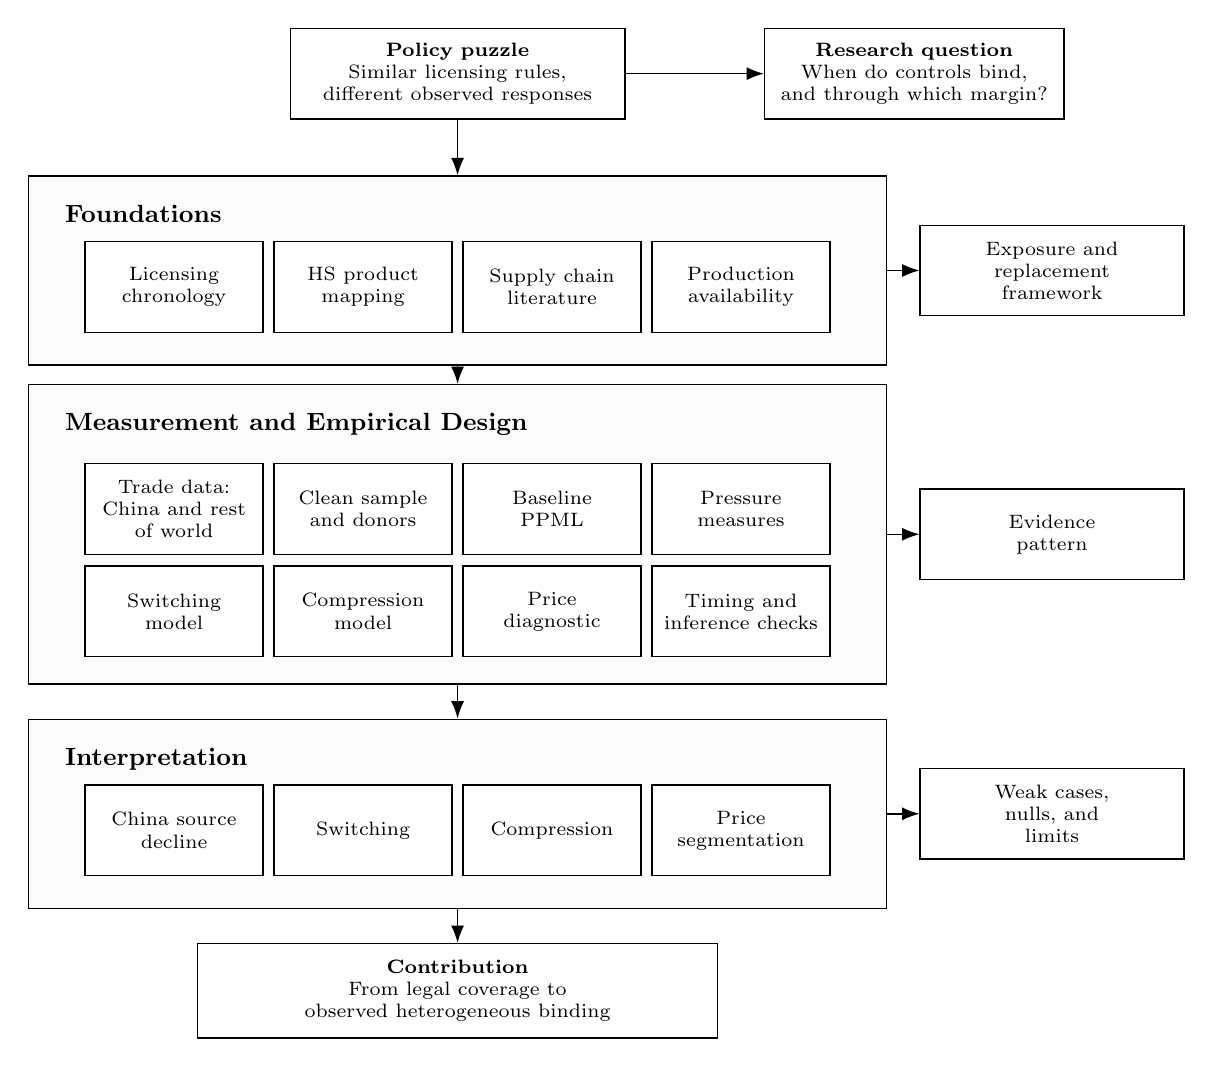
\begin{tikzpicture}[
  font=\scriptsize,
  group/.style={draw, line width=0.55pt, fill=gray!3},
  title/.style={font=\bfseries\small, anchor=north west},
  ibox/.style={draw, line width=0.5pt, align=center, inner sep=3pt, minimum width=2.25cm, minimum height=1.15cm, text width=2.05cm, fill=white},
  topbox/.style={draw, line width=0.5pt, align=center, inner sep=4pt, minimum width=4.25cm, minimum height=1.15cm, text width=3.95cm, fill=white},
  sidebox/.style={draw, line width=0.5pt, align=center, inner sep=4pt, minimum width=3.35cm, minimum height=1.15cm, text width=3.05cm, fill=white},
  finalbox/.style={draw, line width=0.55pt, align=center, inner sep=5pt, minimum width=6.6cm, minimum height=1.2cm, text width=6.2cm, fill=white},
  arrow/.style={-{Latex[length=2.2mm]}, line width=0.55pt}
]
\node[topbox] (puzzle) at (0,0.85) {\textbf{Policy puzzle}\\Similar licensing rules,\\different observed responses};
\node[sidebox, minimum width=3.8cm, text width=3.45cm] (rq) at (5.8,0.85) {\textbf{Research question}\\When do controls bind,\\and through which margin?};
\draw[arrow] (puzzle.east) -- (rq.west);

\node[group, minimum width=10.9cm, minimum height=2.4cm] (found) at (0,-1.65) {};
\node[title] at ([xshift=3.5mm,yshift=-2.5mm]found.north west) {Foundations};
\node[ibox] (chron) at (-3.6,-1.86) {Licensing\\chronology};
\node[ibox] (map) at (-1.2,-1.86) {HS product\\mapping};
\node[ibox] (lit) at (1.2,-1.86) {Supply chain\\literature};
\node[ibox] (prod) at (3.6,-1.86) {Production\\availability};
\node[sidebox] (framework) at (7.55,-1.65) {Exposure and\\replacement\\framework};

\node[group, minimum width=10.9cm, minimum height=3.8cm] (design) at (0,-5.0) {};
\node[title] at ([xshift=3.5mm,yshift=-2.5mm]design.north west) {Measurement and Empirical Design};
\node[ibox] (trade) at (-3.6,-4.68) {Trade data:\\China and rest\\of world};
\node[ibox] (sample) at (-1.2,-4.68) {Clean sample\\and donors};
\node[ibox] (baseline) at (1.2,-4.68) {Baseline\\PPML};
\node[ibox] (pressure) at (3.6,-4.68) {Pressure\\measures};
\node[ibox] (switchmodel) at (-3.6,-5.98) {Switching\\model};
\node[ibox] (compressmodel) at (-1.2,-5.98) {Compression\\model};
\node[ibox] (pricediag) at (1.2,-5.98) {Price\\diagnostic};
\node[ibox] (timinginf) at (3.6,-5.98) {Timing and\\inference checks};
\node[sidebox] (pattern) at (7.55,-5.0) {Evidence\\pattern};

\node[group, minimum width=10.9cm, minimum height=2.4cm] (interpret) at (0,-8.55) {};
\node[title] at ([xshift=3.5mm,yshift=-2.5mm]interpret.north west) {Interpretation};
\node[ibox] (decline) at (-3.6,-8.76) {China source\\decline};
\node[ibox] (switching) at (-1.2,-8.76) {Switching};
\node[ibox] (compression) at (1.2,-8.76) {Compression};
\node[ibox] (segmentation) at (3.6,-8.76) {Price\\segmentation};
\node[sidebox] (limits) at (7.55,-8.55) {Weak cases,\\nulls, and\\limits};

\node[finalbox] (contribution) at (0,-10.8) {\textbf{Contribution}\\From legal coverage to\\observed heterogeneous binding};

\draw[arrow] (puzzle.south) -- (found.north);
\draw[arrow] (found.east) -- (framework.west);
\draw[arrow] (found.south) -- (design.north);
\draw[arrow] (design.east) -- (pattern.west);
\draw[arrow] (design.south) -- (interpret.north);
\draw[arrow] (interpret.east) -- (limits.west);
\draw[arrow] (interpret.south) -- (contribution.north);
\end{tikzpicture}%
}
\caption{Research Design and Interpretation Route}
\label{fig:pressure-framework}
\caption*{\footnotesize Notes: The figure summarizes the proposal logic from legal licensing coverage to measurement, estimation, interpretation, and contribution. It is a guide to the research design, not an additional estimator. Source: author's design.}
\end{figure}

\subsubsection{Empirical Expectations}

The expectations are product specific. The thesis does not require every product to support every expectation because heterogeneity is the object of study.

\begin{enumerate}
\item \emph{H1: Heterogeneous China source decline.} Clean treated products should show declines in imports from China after the policy, but effects should vary by product. The expected sign is \(\beta<0\) in the average source-contrast PPML model. This is necessary observed disruption evidence, not proof that every legally controlled product binds in the same way.
\item \emph{H2: Exposure heterogeneity.} China source declines should be stronger for importer-product cells with higher China exposure before the policy. The expected sign is \(\theta<0\) on the exposure interaction in the source-contrast model. This supports exposure logic, but it does not by itself identify the adjustment mechanism.
\item \emph{H3: Switching mechanism.} Higher switching pressure should be associated with import increases from other suppliers. The expected sign is \(\gamma_S>0\) in the rest-of-world mechanism model. This is the key test for switching.
\item \emph{H4: Compression pressure.} Higher compression pressure may be associated with lower total imports or price segmentation. The expected signs are \(\kappa_C<0\) in the total import model and \(\delta>0\) in the price-wedge diagnostic.
\item \emph{H5: Price segmentation.} Domestic and international price wedges should widen where licensing pressure creates segmentation or scarcity and benchmarks are comparable. The expected sign is \(\delta>0\) for the international relative to domestic post wedge. The price result is diagnostic evidence only.
\end{enumerate}

\subsection{Variables}

The primary outcome is import value in U.S. dollars at the importer, product, source, and month level, aggregated to quarters for the preferred baseline. The source dimension has two values: China and rest of world (RoW). Additional outcomes separate China imports, RoW imports, and total imports at the importer-product level. Net weight is a robustness outcome only where reporting is reliable.

The main pressure variables are China exposure before the policy, revealed outside access, product-level production availability, replacement feasibility, switching pressure, compression pressure, and raw China pressure. Treatment timing uses product-policy status, China source status, post indicators, and event-time indicators around announcement, implementation, import effect, and first full quarter after implementation anchors.

The price wedge is the log difference between comparable international and Chinese domestic benchmarks after harmonizing unit, currency, grade, location, and quotation basis. It is a price segmentation diagnostic, not proof of license denial or compression.

Table \ref{tab:variables_outcomes} summarizes the main outcomes and pressure variables used in the empirical design.

\begin{table}[htbp]
\caption{Main Outcomes and Pressure Variables}
\label{tab:variables_outcomes}
\centering
\begingroup
\small
\setlength{\tabcolsep}{4pt}
\renewcommand{\arraystretch}{1.08}
\begin{tabularx}{\textwidth}{>{\raggedright\arraybackslash}p{0.22\textwidth}>{\raggedright\arraybackslash}p{0.25\textwidth}>{\raggedright\arraybackslash}X}
\toprule
Block & Measure & Construction \\
\midrule
Primary trade outcome & Import value & U.S. dollar import value by importer, product, source, and time. Monthly records are aggregated to quarters for the preferred baseline. \\
Source margins & China imports; rest of world imports; total imports & China and non-China import values are separated, then summed to measure total importer-product imports. \\
Quantity robustness & Net weight & Reported net weight where complete case coverage is credible. \\
Exposure & China exposure & Importer's China share before treatment, measured within each product. \\
Outside access & Outside supplier access & Capped ratio of imports from other suppliers to imports from China before treatment. \\
External availability & Production availability & Product-level USGS production scale term multiplied by rest of world production diversity. \\
Pressure measures & Replacement feasibility, switching pressure, compression pressure, raw China pressure & Replacement feasibility combines outside access and production availability. Switching pressure is exposed demand with replacement feasibility. Compression pressure is exposed demand with limited replacement feasibility. \\
Timing variables & Treatment, China source, post indicators, event-time indicators & Treatment follows official control scope. Timing anchors include announcement, implementation, import effect, and first full quarter after implementation. \\
Price outcome & Price wedge & Log international price relative to the Chinese domestic benchmark after harmonizing grade, unit, currency, location, and quotation basis. \\
\bottomrule
\end{tabularx}
\caption*{\footnotesize Notes: Pressure variables use trade primitives measured before the policy and product-level production availability. Switching pressure and compression pressure add to China exposure, so their coefficients are diagnostic gradients rather than independent structural parameters.}
\endgroup
\end{table}


\subsection{Data Sources and Processing}

\subsubsection{UN Comtrade Bilateral Imports}

The trade panel uses monthly UN Comtrade bilateral import records from January 2019 through March 2026. The final analysis sample has 53 reporters, 87 months, two source groups, four clean treated products, and 12 donor candidates. Monthly bilateral sources are collapsed into China and rest of world sources. The preferred baseline aggregates monthly observations to quarters because customs reporting, shipping lags, and policy implementation do not map cleanly to exact announcement days. Monthly models remain robustness and timing diagnostics.

The data construction keeps canonical aggregate records for each reporter, product, and month. It excludes transport mode, customs procedure, secondary partner, and duplicate aggregate rows to avoid double counting. HS 3801 is excluded from the main analysis because it is partially treated, and HS 2501 is excluded because it is too sparse.

The main clean treated products are shown in Table \ref{tab:product-scope}. They are HS 2504 natural graphite, HS 8110 antimony metal and articles, HS 8106 bismuth metal, and HS 284180 tungstates/APT. Donor products are retained only after policy status, trade regularity, reporting coverage, and donor suitability screens. The donor products are not treated as close mineral substitutes. They are untreated comparison products used to absorb common reporting, importer, and time shocks in the source contrast design. The final thesis appendix will report the donor list, exclusion rules, trade regularity screens, and PPML separation diagnostics.

\begin{table}[H]
\caption{Clean Treated Products and Policy Timing}
\label{tab:product-scope}
\centering
\begingroup
\let\proposaloldsmall\small
\renewcommand{\small}{\scriptsize}
\setlength{\tabcolsep}{2pt}
\renewcommand{\arraystretch}{1.08}
\begin{tabularx}{\textwidth}{>{\raggedright\arraybackslash}p{0.07\textwidth}>{\raggedright\arraybackslash}p{0.16\textwidth}>{\raggedright\arraybackslash}p{0.10\textwidth}>{\centering\arraybackslash}p{0.145\textwidth}>{\centering\arraybackslash}p{0.145\textwidth}>{\centering\arraybackslash}p{0.145\textwidth}>{\raggedright\arraybackslash}X}
\toprule
HS code & Product & Policy wave & Announcement & Implementation & Import effect month & Sample status \\
\midrule
2504 & Natural graphite & Graphite & \mbox{2023-10-20} & \mbox{2023-12-01} & \mbox{2024-01} & Clean baseline product \\
8110 & Antimony metal and articles & Antimony & \mbox{2024-08-15} & \mbox{2024-09-15} & \mbox{2024-10} & Clean baseline product \\
8106 & Bismuth metal & W/Bi group & \mbox{2025-02-04} & \mbox{2025-02-04} & \mbox{2025-03} & Clean baseline product \\
284180 & Tungstates/APT & W/Bi group & \mbox{2025-02-04} & \mbox{2025-02-04} & \mbox{2025-03} & Clean baseline product \\
\bottomrule
\end{tabularx}
\caption*{\footnotesize Notes: The table lists the four clean treated products used in the main baseline. Legal coverage and clean HS mapping do not by themselves imply observed binding. Source: official policy chronology and author sample construction.}
\endgroup
\end{table}


\subsubsection{Product Mapping and HS Observability}

Product mapping connects legal control lists to trade data. The main baseline uses only four clean treated products, but clean legal mapping does not guarantee a strong empirical effect. HS 2504 records natural graphite, with remaining caveats about graphite grades and earlier control history. HS 8110 records antimony metal and articles, while the production proxy is upstream antimony mine output. HS 8106 records bismuth metal, with byproduct and refining constraints. HS 284180 records tungstates and APT, but the production proxy is upstream tungsten mine output.

Bundled, partial, and sparse products can still be useful as excluded context or thesis appendix diagnostics. They do not carry the main baseline interpretation. An HS-level null does not prove that every legally controlled item is unaffected. Conversely, a legally clean mapping does not imply observed binding. Tungstates/APT are legally clean in the baseline but empirically weak, null, or unresolved.

\subsubsection{Production-Based External Availability}

The production-based availability measure uses USGS \emph{Mineral Commodity Summaries 2025} world production data, with 2023 as the baseline and 2024 as robustness \citep{usgs_mcs_2025}. Table \ref{tab:production-availability} reports the compact construction used in the proposal. Production is external availability, not spare short-run capacity. The production mapping is strongest for graphite, useful but upstream for antimony and tungsten, and constrained for bismuth because bismuth is tied to refining and byproduct economics.

\begin{table}[H]
\caption{USGS Production Availability Measures}
\label{tab:production-availability}
\centering
\begingroup
\footnotesize
\setlength{\tabcolsep}{4pt}
\renewcommand{\arraystretch}{1.05}
\begin{tabularx}{\textwidth}{>{\raggedright\arraybackslash}p{0.09\textwidth}>{\raggedright\arraybackslash}p{0.23\textwidth}>{\raggedleft\arraybackslash}p{0.14\textwidth}>{\raggedleft\arraybackslash}p{0.14\textwidth}>{\raggedright\arraybackslash}X}
\toprule
HS code & Product & 2023 \(A^{prod}\) & 2024 \(A^{prod}\) & Mapping caveat \\
\midrule
2504 & Natural graphite & 0.216 & 0.219 & Direct production proxy \\
8110 & Antimony metal & 0.519 & 0.494 & Upstream production proxy \\
8106 & Bismuth metal & 0.152 & 0.166 & Refinery and byproduct caveat \\
284180 & Tungstates/APT & 0.176 & 0.182 & Upstream tungsten proxy \\
\bottomrule
\end{tabularx}
\caption*{\footnotesize Notes: \(A^{prod}=Scale^{prod}\times(1-HHI^{ROW,prod})\). Detailed production, scale, HHI, diversity, and country rows are reserved for the thesis appendix; the main proposal uses this compact version to avoid overcrowding. Source: author calculations from USGS \emph{Mineral Commodity Summaries 2025} world production data \citep{usgs_mcs_2025}.}
\endgroup
\end{table}


\subsubsection{Domestic and International Price Benchmarks}

Domestic and international price benchmarks enter as diagnostic evidence. The price variables compare international and Chinese domestic benchmarks after harmonizing grade, unit, currency, location, and quotation basis as far as the data allow. The identifying object is a domestic and international wedge, not a license approval outcome, export denial, or welfare measure.

Antimony and bismuth have the strongest usable price-wedge evidence in the preliminary empirical evidence. Graphite is exploratory and weak because the international benchmark description is not fully documented. Tungsten/APT is not supportive: the benchmark is description sensitive and the observed wedge moves in the wrong direction for a segmentation claim. Price wedges are therefore used only as evidence consistent with segmentation or scarcity. They do not prove license denial, total import compression, or the internal licensing channel.

\subsubsection{Demand, Market Structure, and Geographic Context Variables}

Demand, market structure, and geographic variables help discipline interpretation and auxiliary robustness. Relevant context includes importer demand conditions, downstream use intensity, supplier concentration before the policy, product-level production concentration, distance and regional sourcing patterns, and the presence of established non-China suppliers. These variables help distinguish a licensing response from broader demand changes, commodity cycle movements, or measurement differences across HS codes.

These context variables are not mechanically included in the baseline PPML specification. Importer time fixed effects absorb many importer wide demand shocks, product time fixed effects absorb common product shocks, and importer product fixed effects absorb persistent bilateral sourcing structure. Some contextual variables are also measured after treatment, collinear with the fixed effects, or too coarse to enter the main model without changing the estimand. They are therefore used to interpret product patterns, motivate robustness checks, and organize thesis appendix evidence rather than to replace the baseline source-contrast design.

\subsection{Empirical Strategy and Model}

The empirical hierarchy is set before interpretation. Quarterly PPML is the preferred baseline. Monthly models are robustness and timing diagnostics. Interpretation is by product. Pooled clean estimates are summary evidence only because pooled pretrends fail. Event studies and placebo tests are diagnostics, not proof of clean causal timing.

\subsubsection{Baseline China Source Response}

The first empirical object is the average change in China source imports for treated products. The model compares China sourcing with rest of world sourcing, before and after the relevant licensing date, while controlling for importer, product, source, and time structure:
\begin{equation}
\begin{aligned}
\mathbb{E}\left[M_{ipst}\mid X_{ipst}\right]
&=\exp\Bigl[
\beta D_{pst}
+\alpha_{ips}
+\delta_{it}
+\lambda_{pt}
+\mu_{st}
\Bigr]
\end{aligned}
\end{equation}
where
\begin{equation}
D_{pst}=Treated_p\times China_s\times Post_{pt}
\end{equation}
\(M_{ipst}\) is import value. \(China_s\) equals one for Chinese origin imports and zero for rest of world imports. \(Post_{pt}\) follows product-policy timing. The fixed effects absorb importer product source relationships, importer time shocks, product time shocks, and source time shocks. The expected sign is \(\beta<0\). The coefficient estimates a China source shift relative to other sources and donor products; it does not prove license denial.

\subsubsection{Pressure Measures in the China Source Model}

A simpler exposure specification interacts treatment with China exposure before the policy:
\begin{equation}
\begin{aligned}
\mathbb{E}\left[M_{ipst}\mid X_{ipst}\right]
&=\exp\Bigl[
\beta D_{pst}
+\theta\left(D_{pst}\times E_{ip}\right)
+\alpha_{ips}
+\delta_{it}
+\lambda_{pt}
+\mu_{st}
\Bigr]
\end{aligned}
\end{equation}
The expected sign is \(\theta<0\): China source declines should be larger where the importer depended more on China before the policy. This model tests exposure logic, but it does not identify the adjustment mechanism.

The main pressure specification separates switching pressure and compression pressure:
\begin{equation}
\begin{aligned}
\mathbb{E}\left[M_{ipst}\mid X_{ipst}\right]
&=\exp\Bigl[
\beta D_{pst}
+\theta_S\left(D_{pst}\times P^S_{ip}\right)
+\theta_C\left(D_{pst}\times P^C_{ip}\right) \\
&\qquad
+\alpha_{ips}
+\delta_{it}
+\lambda_{pt}
+\mu_{st}
\Bigr]
\end{aligned}
\end{equation}
The expected signs are \(\theta_S<0\) and \(\theta_C<0\). This model asks whether the pressure measures predict stronger China source decline. It does not by itself show whether the adjustment came from switching or compression, because both margins can reduce China sourcing.

\subsubsection{Switching Mechanism}

The switching model uses imports from all non-China suppliers as the outcome:
\begin{equation}
\begin{aligned}
\mathbb{E}\left[M^R_{ipt}\mid X_{ipt}\right]
&=\exp\Bigl[
\gamma_S\left(Treated_p\times Post_{pt}\times P^S_{ip}\right)
+\gamma_C\left(Treated_p\times Post_{pt}\times P^C_{ip}\right) \\
&\qquad
+\alpha_{ip}
+\delta_{it}
+\lambda_{pt}
\Bigr]
\end{aligned}
\end{equation}
The key expected sign is \(\gamma_S>0\). A positive coefficient on switching pressure is evidence consistent with replacement of Chinese supply by other suppliers. It is not evidence of compression.

\subsubsection{Total Import Compression}

The compression model uses total imports from all sources:
\begin{equation}
\begin{aligned}
\mathbb{E}\left[M^{Total}_{ipt}\mid X_{ipt}\right]
&=\exp\Bigl[
\kappa_C\left(Treated_p\times Post_{pt}\times P^C_{ip}\right)
+\kappa_S\left(Treated_p\times Post_{pt}\times P^S_{ip}\right) \\
&\qquad
+\alpha_{ip}
+\delta_{it}
+\lambda_{pt}
\Bigr]
\end{aligned}
\end{equation}
The key expected sign is \(\kappa_C<0\). Compression is supported only when total imports decline with compression pressure. It is not inferred mechanically from a China source decline.

\subsubsection{Price Wedge Diagnostic}

For comparable price pairs, the diagnostic price model is:
\begin{equation}
\begin{aligned}
\log P_{rpt}
&=\alpha_{rp}
+\lambda_t
+\delta\left(International_r\times Post_{pt}\right)
+\varepsilon_{rpt}
\end{aligned}
\end{equation}
\(P_{rpt}\) is the benchmark price for region or quotation basis \(r\), product \(p\), and time \(t\). \(International_r\) equals one for the international benchmark and zero for the Chinese domestic benchmark. The expected sign is \(\delta>0\) for a widening international relative to domestic wedge. This is diagnostic evidence consistent with scarcity or segmentation. It is not causal proof of licensing denial or compression.

\subsubsection{Timing, Placebo, and Robustness Checks}

Event studies replace the post indicator with event-time indicators:
\begin{equation}
\begin{aligned}
\mathbb{E}\left[M_{ipst}\mid X_{ipst}\right]
&=\exp\Biggl[
\sum_{k\neq -1}\beta_k
\left(Treated_p\times China_s\times 1\{EventTime_{pt}=k\}\right) \\
&\qquad
+\alpha_{ips}
+\delta_{it}
+\lambda_{pt}
+\mu_{st}
\Biggr]
\end{aligned}
\end{equation}
\(EventTime_{pt}\) indexes time relative to the product-policy anchor, with \(k=-1\) omitted. Event studies are timing and pretrend diagnostics only. Coefficients before the policy should not systematically differ from zero, and persistent movement after the policy is more persuasive than a one-period break. Failed pretrends weaken timing claims. Missing event study outputs are unavailable diagnostics, not passes.

Placebo tests construct fake treatment timing before actual controls:
\begin{equation}
D^{placebo}_{pst}=Treated_p\times China_s\times PlaceboPost_{pt}
\end{equation}
\(PlaceboPost_{pt}\) equals one after the placebo policy date and before the true policy date. Significant placebo effects weaken timing interpretation. Robustness checks include U.S.-excluded samples, net weight outcomes where quantity reporting is reliable, alternative timing anchors, production-\(A\) 2024 variants, and monthly specifications. These checks support interpretation only when they are consistent with the quarterly baseline and mechanism evidence.

\subsection{Preliminary Empirical Evidence}

\subsubsection{China Source Response}

The preferred preliminary evidence starts with quarterly PPML estimates using the first full quarter after implementation timing anchor. Table \ref{tab:china-source-response} reports the average China source response and the China source pressure specifications by product. Antimony metal and bismuth metal have the strongest average declines in imports from China. Natural graphite is negative but weaker. Tungstates/APT are weak or null in the average China source row.

The pressure rows are useful because they ask whether observed declines are stronger where the framework predicts more exposure or harder replacement. Natural graphite has a negative China exposure coefficient and a negative compression pressure coefficient. Bismuth has a negative compression pressure coefficient, but the broader quantity mechanism evidence is less precise. Tungstates/APT show a negative exposure coefficient but do not show a persuasive average decline, so the pressure row is not treated as a positive product case. The pooled clean estimate is negative, but because pooled pretrends fail, it is used only as summary evidence. Interpretation rests on the product results.

Full model outputs in the thesis appendix will report observations, separated observations, dropped fixed-effect cells, and convergence warnings.

\providecommand{\estcell}[2]{\begin{tabular}[c]{@{}c@{}}#1\\(#2)\end{tabular}}

\begin{table}[H]
\caption{China Source Response}
\label{tab:china-source-response}
\centering
\begingroup
\footnotesize
\setlength{\tabcolsep}{4pt}
\renewcommand{\arraystretch}{1.16}
\begin{tabularx}{\textwidth}{>{\raggedright\arraybackslash}p{0.24\textwidth}>{\centering\arraybackslash}X>{\centering\arraybackslash}X>{\centering\arraybackslash}X>{\centering\arraybackslash}X}
\toprule
Model & Natural graphite & Antimony metal & Bismuth metal & Tungstates/APT \\
\midrule
Average China source effect & \estcell{-30.1*}{-1.77} & \estcell{-86.7***}{-5.75} & \estcell{-74.4***}{-3.61} & \estcell{-15.2}{-0.41} \\
China exposure & \estcell{-0.364***}{-4.06} & \estcell{-0.179}{-0.47} & \estcell{-0.584}{-1.55} & \estcell{-0.363***}{-2.71} \\
Switching pressure & \estcell{0.191}{1.04} & \estcell{-0.078}{-0.23} & \estcell{-0.195}{-0.44} & \estcell{0.156}{1.17} \\
Compression pressure & \estcell{-0.218**}{-2.02} & \estcell{-0.128}{-0.80} & \estcell{-0.593**}{-1.97} & \estcell{-0.183}{-0.83} \\
\bottomrule
\end{tabularx}
\caption*{\footnotesize Notes: The average China source effect is reported as a percent effect from the PPML coefficient. Other rows report pressure interaction coefficients from the preferred quarterly production-\(A\) China source specifications. Parentheses report \(t\)-statistics computed from reported standard errors. Stars use reported \(p\)-values: * \(p<0.10\), ** \(p<0.05\), *** \(p<0.01\). Standard errors are clustered by reporter code.}
\endgroup
\end{table}


The pressure rows in Table \ref{tab:china-source-response} are diagnostic China source gradients. They do not identify switching or compression by themselves; the mechanism interpretation comes from the rest of world and total import models in Table \ref{tab:adjustment-mechanisms} and the price evidence in Table \ref{tab:price-diagnostics}.

\subsubsection{Adjustment Mechanisms}

Table \ref{tab:adjustment-mechanisms} separates the two quantity mechanisms.

\providecommand{\estcell}[2]{\begin{tabular}[c]{@{}c@{}}#1\\(#2)\end{tabular}}

\begin{table}[H]
\caption{Adjustment Mechanisms}
\label{tab:adjustment-mechanisms}
\centering
\begingroup
\footnotesize
\setlength{\tabcolsep}{4pt}
\renewcommand{\arraystretch}{1.16}
\begin{tabularx}{\textwidth}{>{\raggedright\arraybackslash}p{0.24\textwidth}>{\centering\arraybackslash}X>{\centering\arraybackslash}X>{\centering\arraybackslash}X>{\centering\arraybackslash}X}
\toprule
Mechanism & Natural graphite & Antimony metal & Bismuth metal & Tungstates/APT \\
\midrule
Rest of world switching & \estcell{0.342***}{2.59} & \estcell{0.405***}{3.42} & \estcell{0.196}{1.38} & \estcell{0.161}{1.06} \\
Total import compression & \estcell{-0.165**}{-2.03} & \estcell{0.287}{1.38} & \estcell{-0.134}{-0.66} & \estcell{0.441***}{3.63} \\
\bottomrule
\end{tabularx}
\caption*{\footnotesize Notes: Entries are pressure interaction coefficients from the preferred quarterly production-\(A\) mechanism specifications. Parentheses report \(t\)-statistics computed from reported standard errors. Stars use reported \(p\)-values: * \(p<0.10\), ** \(p<0.05\), *** \(p<0.01\). Standard errors are clustered by reporter code.}
\endgroup
\end{table}


Rest of world switching is the broadest mechanism. The switching coefficient is positive for all four products and is strongest for natural graphite and antimony metal. This pattern is consistent with replacement of Chinese supply by other suppliers, but it does not show that total imports were fully protected from disruption.

Compression is narrower. Natural graphite is the only product with a negative and statistically supported total import compression coefficient in the preferred compression row. Bismuth has the expected sign but is imprecise. Antimony metal and tungstates/APT move in the opposite direction for a compression claim. Compression therefore remains product specific rather than a general conclusion.

\subsubsection{Price Diagnostics}

Table \ref{tab:price-diagnostics} reports the price-wedge diagnostic.

\providecommand{\estcell}[2]{\begin{tabular}[c]{@{}c@{}}#1\\(#2)\end{tabular}}

\begin{table}[H]
\caption{Price Diagnostics}
\label{tab:price-diagnostics}
\centering
\begingroup
\footnotesize
\setlength{\tabcolsep}{4pt}
\renewcommand{\arraystretch}{1.16}
\begin{tabularx}{\textwidth}{>{\raggedright\arraybackslash}p{0.24\textwidth}>{\centering\arraybackslash}X>{\centering\arraybackslash}X>{\centering\arraybackslash}X>{\centering\arraybackslash}X}
\toprule
Diagnostic & Natural graphite & Antimony metal & Bismuth metal & Tungstates/APT \\
\midrule
Price wedge & \estcell{-0.067*}{-1.84} & \estcell{0.460***}{3.88} & \estcell{0.837***}{6.72} & \estcell{-0.115**}{-2.11} \\
\bottomrule
\end{tabularx}
\caption*{\footnotesize Notes: Entries are log point changes in international prices relative to Chinese domestic benchmarks from the price-wedge diagnostics. Parentheses report \(t\)-statistics computed from reported standard errors. Stars use reported \(p\)-values: * \(p<0.10\), ** \(p<0.05\), *** \(p<0.01\). The source price models use reported HAC(3) standard errors rather than reporter clustering. Price-wedge estimates are diagnostic and do not identify license denials, compression, or welfare effects.}
\endgroup
\end{table}


Antimony metal and bismuth metal have positive and precisely estimated coefficients, which supports a price segmentation interpretation. Graphite's price wedge is negative and only marginally estimated, so it does not support positive price segmentation. Tungstates/APT also move in the wrong direction for a positive segmentation claim. These price results are diagnostic; they do not prove license denial, total import compression, welfare loss, or the internal licensing channel.

\subsubsection{Timing and Product Interpretation}

Timing evidence is treated as a diagnostic layer rather than as clean causal identification. No event study figure is shown because no final product-level event study is clean enough for main-text display without risking an overclaim about timing. A bismuth or graphite timing figure is not used as main evidence because the product-level interpretation is clearer in the quarterly baseline tables, and the pressure event diagnostics remain weak or incomplete. Missing monthly diagnostics are unavailable evidence, not passing checks.

The timing and robustness hierarchy is therefore as follows. Pooled pretrends fail, so pooled estimates are summary only. Graphite average timing is acceptable, but pressure event diagnostics are weak. Antimony metal is substantively strong but has timing and placebo caveats. Bismuth has stronger average and price evidence, but weaker quantity mechanisms. Tungstates/APT have bad timing and placebo diagnostics.

The final product classification is unchanged. Natural graphite has a moderate average decline, clear switching and compression evidence in the quarterly mechanism models, and no positive price segmentation. Antimony metal has the strongest observed disruption, strong switching and price segmentation, no compression support, and a timing and placebo caveat. Bismuth metal has a strong average decline and strong price segmentation, with weaker quantity mechanism evidence. Tungstates/APT are weak, null, or unresolved, with bad timing and placebo diagnostics; this case is useful evidence that clean legal coverage does not imply observed binding.

\subsection{Research Structure}

The thesis will proceed in six parts. The introduction will state the heterogeneous binding puzzle, research question, and contribution. The background chapter will reconstruct China's licensing chronology, legal basis, product scope, and timing. The theory chapter will develop the exposure and replacement framework. The data chapter will document Comtrade construction, clean product mapping, donor screening, production availability, price benchmarks, and contextual variables. The empirical chapter will present quarterly source-contrast PPML results, pressure interactions, rest of world switching, total import compression, price wedges, timing diagnostics, placebo tests, and robustness checks. The final chapter will interpret the product evidence and limitations.

The structure keeps legal coverage, observed binding, source switching, compression, and price segmentation separate. This separation is the main guard against overstating the thesis as a clean causal treatment effect paper.

\section{Contributions, Innovations, and Limitations}

\subsection{Academic Contributions}

The thesis makes three academic contributions. First, it separates legal licensing coverage from observed binding response. This distinction matters because a license requirement can be legally active while producing weak or undetected HS-level market movement. The thesis therefore treats binding as an observed response in trade or price data, not as a synonym for legal coverage.

Second, the thesis separates exposure from replacement feasibility. Concentration and China source dependence describe potential pressure, but they do not show whether importers can replace Chinese supply. The pressure framework combines China exposure before the policy, importer outside access, and production-based external availability. This design uses product-level production data rather than trade outcomes after the policy, while keeping clear that production is not spare short-run capacity.

Third, the thesis classifies mechanisms by product instead of ranking products by one average effect. The empirical design distinguishes China source decline, rest of world switching, total import compression, price segmentation, and weak or null response. This allows the thesis to interpret graphite as mixed switching and compression, antimony as strong disruption with switching and price segmentation but timing caveats, bismuth as strong disruption with price segmentation and weaker quantity mechanisms, and tungstates/APT as weak, null, or unresolved.

\subsection{Policy Contributions}

The policy contribution is to evaluate China's licensing controls through observed market response rather than through announcement counts. A control can be legally active and still show no detected aggregate HS-level China source decline. Another control can produce a large source shift in a cleaner product code. Policy evaluation should therefore track legal timing and measured trade or price response separately.

HS code mapping matters for policy interpretation. Broad HS codes can mix controlled and uncontrolled items. Sparse codes can produce unstable estimates. A clean code can still produce weak results. This proposal uses product mapping to decide what each estimate can and cannot say.

Different response margins imply different policy lessons. Rest of world switching means foreign importers can redirect some demand away from China. Total import compression means exposed importers do not replace enough supply in observed trade values. Price segmentation means pressure may appear in domestic and international price gaps even when quantities do not clearly contract. The thesis does not estimate welfare, coercive success, or license denial, but it can show which observable margin moves after a licensing control.

\subsection{Research Limitations}

The proposed study has clear measurement limits. Monthly customs data observe HS-level trade values, not license applications, approvals, denials, processing times, customs communications, firm contracts, inventories, or downstream production effects. A negative China source estimate can show an observed market response, but it cannot identify the internal licensing channel that generated that response.

The pressure measures are proxies. China exposure and outside access are trade primitives measured before the policy. Production availability measures product-level external production, not spare short-run export capacity. Switching pressure and compression pressure are proxy decompositions, not structural parameters, and their identity with China exposure limits independent coefficient interpretation. Antimony and tungsten use upstream production proxies. Bismuth has byproduct and refining constraints.

HS code mapping limits interpretation. Clean and regularly traded codes can support stronger claims than bundled, partial, or sparse codes, but even clean legal mapping does not guarantee a strong observed effect. Tungstates/APT are legally clean but empirically weak, null, or unresolved. An HS-level null should not be read as proof that every legally controlled item was unaffected.

The main outcome is import value rather than physical quantity. Import values are available more consistently across reporters and products, but they combine price, quantity, quality, and composition. Net weight data are robustness evidence only where complete case coverage is credible. Price wedges have a narrow role and are used only when benchmark pairs match on grade, unit, currency, location, and quotation basis.

The timing and inference problems are structural to the design. Quarterly aggregation is the preferred baseline because monthly customs data are noisy and policy implementation does not map cleanly to exact days. Treatment varies at the product and time level, while the panel contains many reporter and time observations. Reporter clustered p values are useful conditional diagnostics, but they do not create many independent policy shocks. PPML separation drops observations in many models. There are few treated products and few product-policy shocks, and pooled pretrends fail.

Timing diagnostics remain important caveats. Antimony has strong observed disruption, switching, and price-wedge evidence, but its placebo and timing diagnostics are problematic. Tungstates/APT have weak or opposite signed mechanism evidence and bad timing and placebo diagnostics. Monthly event study and placebo diagnostics are incomplete in some blocks. Missing or failed diagnostics are treated as unavailable diagnostics, not as evidence that timing checks pass.

For these reasons, the thesis uses mechanism consistent and heterogeneous binding language rather than clean causal treatment effect language. The estimates identify observed trade and price responses consistent with heterogeneous binding pressure. They do not identify license applications, approvals, denials, processing delays, welfare losses, coercive success, or clean causal timing.

\section{Research Plan and Timeline}

The remaining work is to integrate the evidence into the full thesis manuscript, document robustness checks, organize appendices, and keep interpretation within the limits of the design. The thesis will not be expanded into a broader welfare or coercive success study. The empirical chapter will present the quarterly baseline first, followed by mechanisms by product, price diagnostics, monthly robustness and timing checks, and model warnings.

Appendix material will document full regression rows, PPML separation drops, missing or failed event study and placebo blocks, U.S.-excluded checks, net weight robustness, and production-\(A\) 2024 variants. Product classifications will be checked against the interpretation used in the proposal: graphite as mixed switching and compression, antimony as strong disruption with switching and price segmentation but timing caveats, bismuth as strong disruption with price segmentation and weaker quantity mechanisms, and tungstates/APT as weak, null, or unresolved.

The research plan in Table \ref{tab:timeline} focuses on thesis completion, robustness documentation, supervisor revision, and defense preparation.

\begin{table}[H]
\caption{Thesis Completion Timeline}
\label{tab:timeline}
\centering
\begingroup
\scriptsize
\setlength{\tabcolsep}{3pt}
\renewcommand{\arraystretch}{1.05}
\begin{tabularx}{\textwidth}{>{\raggedright\arraybackslash}p{0.17\textwidth}>{\raggedright\arraybackslash}p{0.31\textwidth}>{\raggedright\arraybackslash}p{0.27\textwidth}>{\raggedright\arraybackslash}X}
\toprule
Period & Task & Output & Constraint \\
\midrule
July 2026 & Integrate proposal tables and figures into the thesis manuscript. & Main result tables, mechanism summary, and pressure framework figure. & Product classifications must match the proposal interpretation. \\
Aug. 2026 & Organize appendix evidence. & Full regression rows, robustness tables, model notes, and missing diagnostic notes. & Missing rows are unavailable diagnostics, not passing checks. \\
Sep. 2026 & Complete robustness and model warning documentation. & U.S.-excluded, net weight, monthly timing, placebo, event study, and production-based \(A\) 2024 appendix notes. & Robustness does not override weak timing or mechanism evidence. \\
Oct. 2026 & Review claims and citations before supervisor circulation. & Claim checklist, citation issue list, and revised interpretation language. & No license denial, welfare, coercive success, or clean causal timing claims. \\
Nov.--Dec. 2026 & Supervisor revision and manuscript tightening. & Revised full thesis and response checklist. & Keep the quarterly baseline and product interpretation central. \\
Jan.--Feb. 2027 & Prepare defense materials. & Defense slides, result handout, and anticipated question notes. & Slides must distinguish legal coverage, observed response, switching, compression, and price segmentation. \\
Mar. 2027 & Final formatting and submission check. & ZJU formatted final manuscript and submitted files. & Check tables, figures, references, equations, and front matter before submission. \\
\bottomrule
\end{tabularx}
\caption*{\footnotesize Notes: The timeline focuses on thesis completion, documentation, revision, and defense preparation.}
\endgroup
\end{table}


\clearpage
\bibliographystyle{plainnat}
\IfFileExists{references.bib}{%
  \bibliography{references}%
}{%
  \IfFileExists{../../02_literature/references.bib}{%
    \bibliography{../../02_literature/references}%
  }{%
    % No bibliography file found. In Overleaf, upload the project bibliography
    % as references.bib when citations are added.
  }%
}

\end{document}
